
\subsection{NVE} %----------------------------------------------------------------------------------------------------------------------------
\begin{frame}{Simulazione NVE}
            
\begin{columns}[c]        
	% Colonna Sinistra: Testo
	\begin{column}{0.48\textwidth}
		
		\centering
		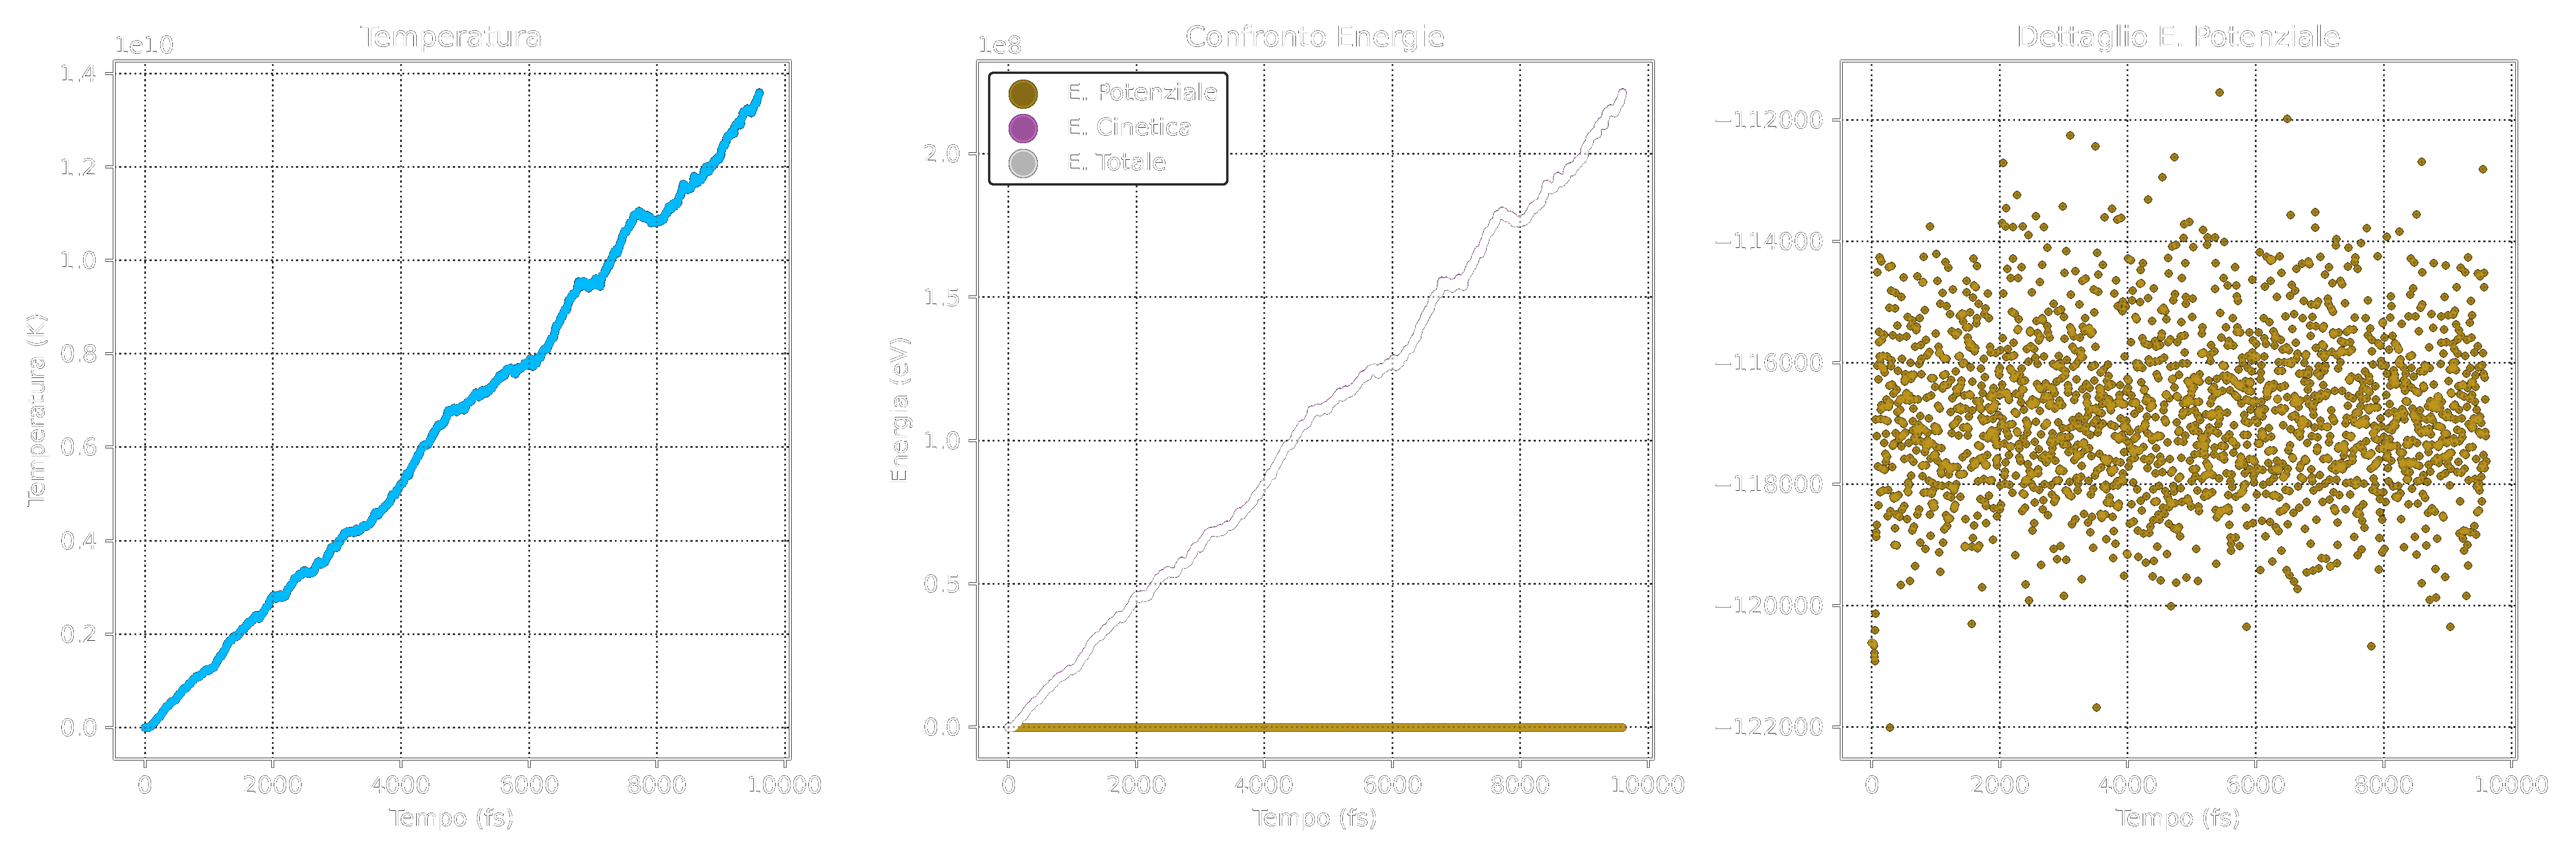
\includegraphics[scale=0.15]{./invnobg/andamento_energia_nve_testdata.png}
		
	\end{column}
	% Colonna Destra: Due immagini incolonnate
	\begin{column}{0.48\textwidth}
		
		\centering
		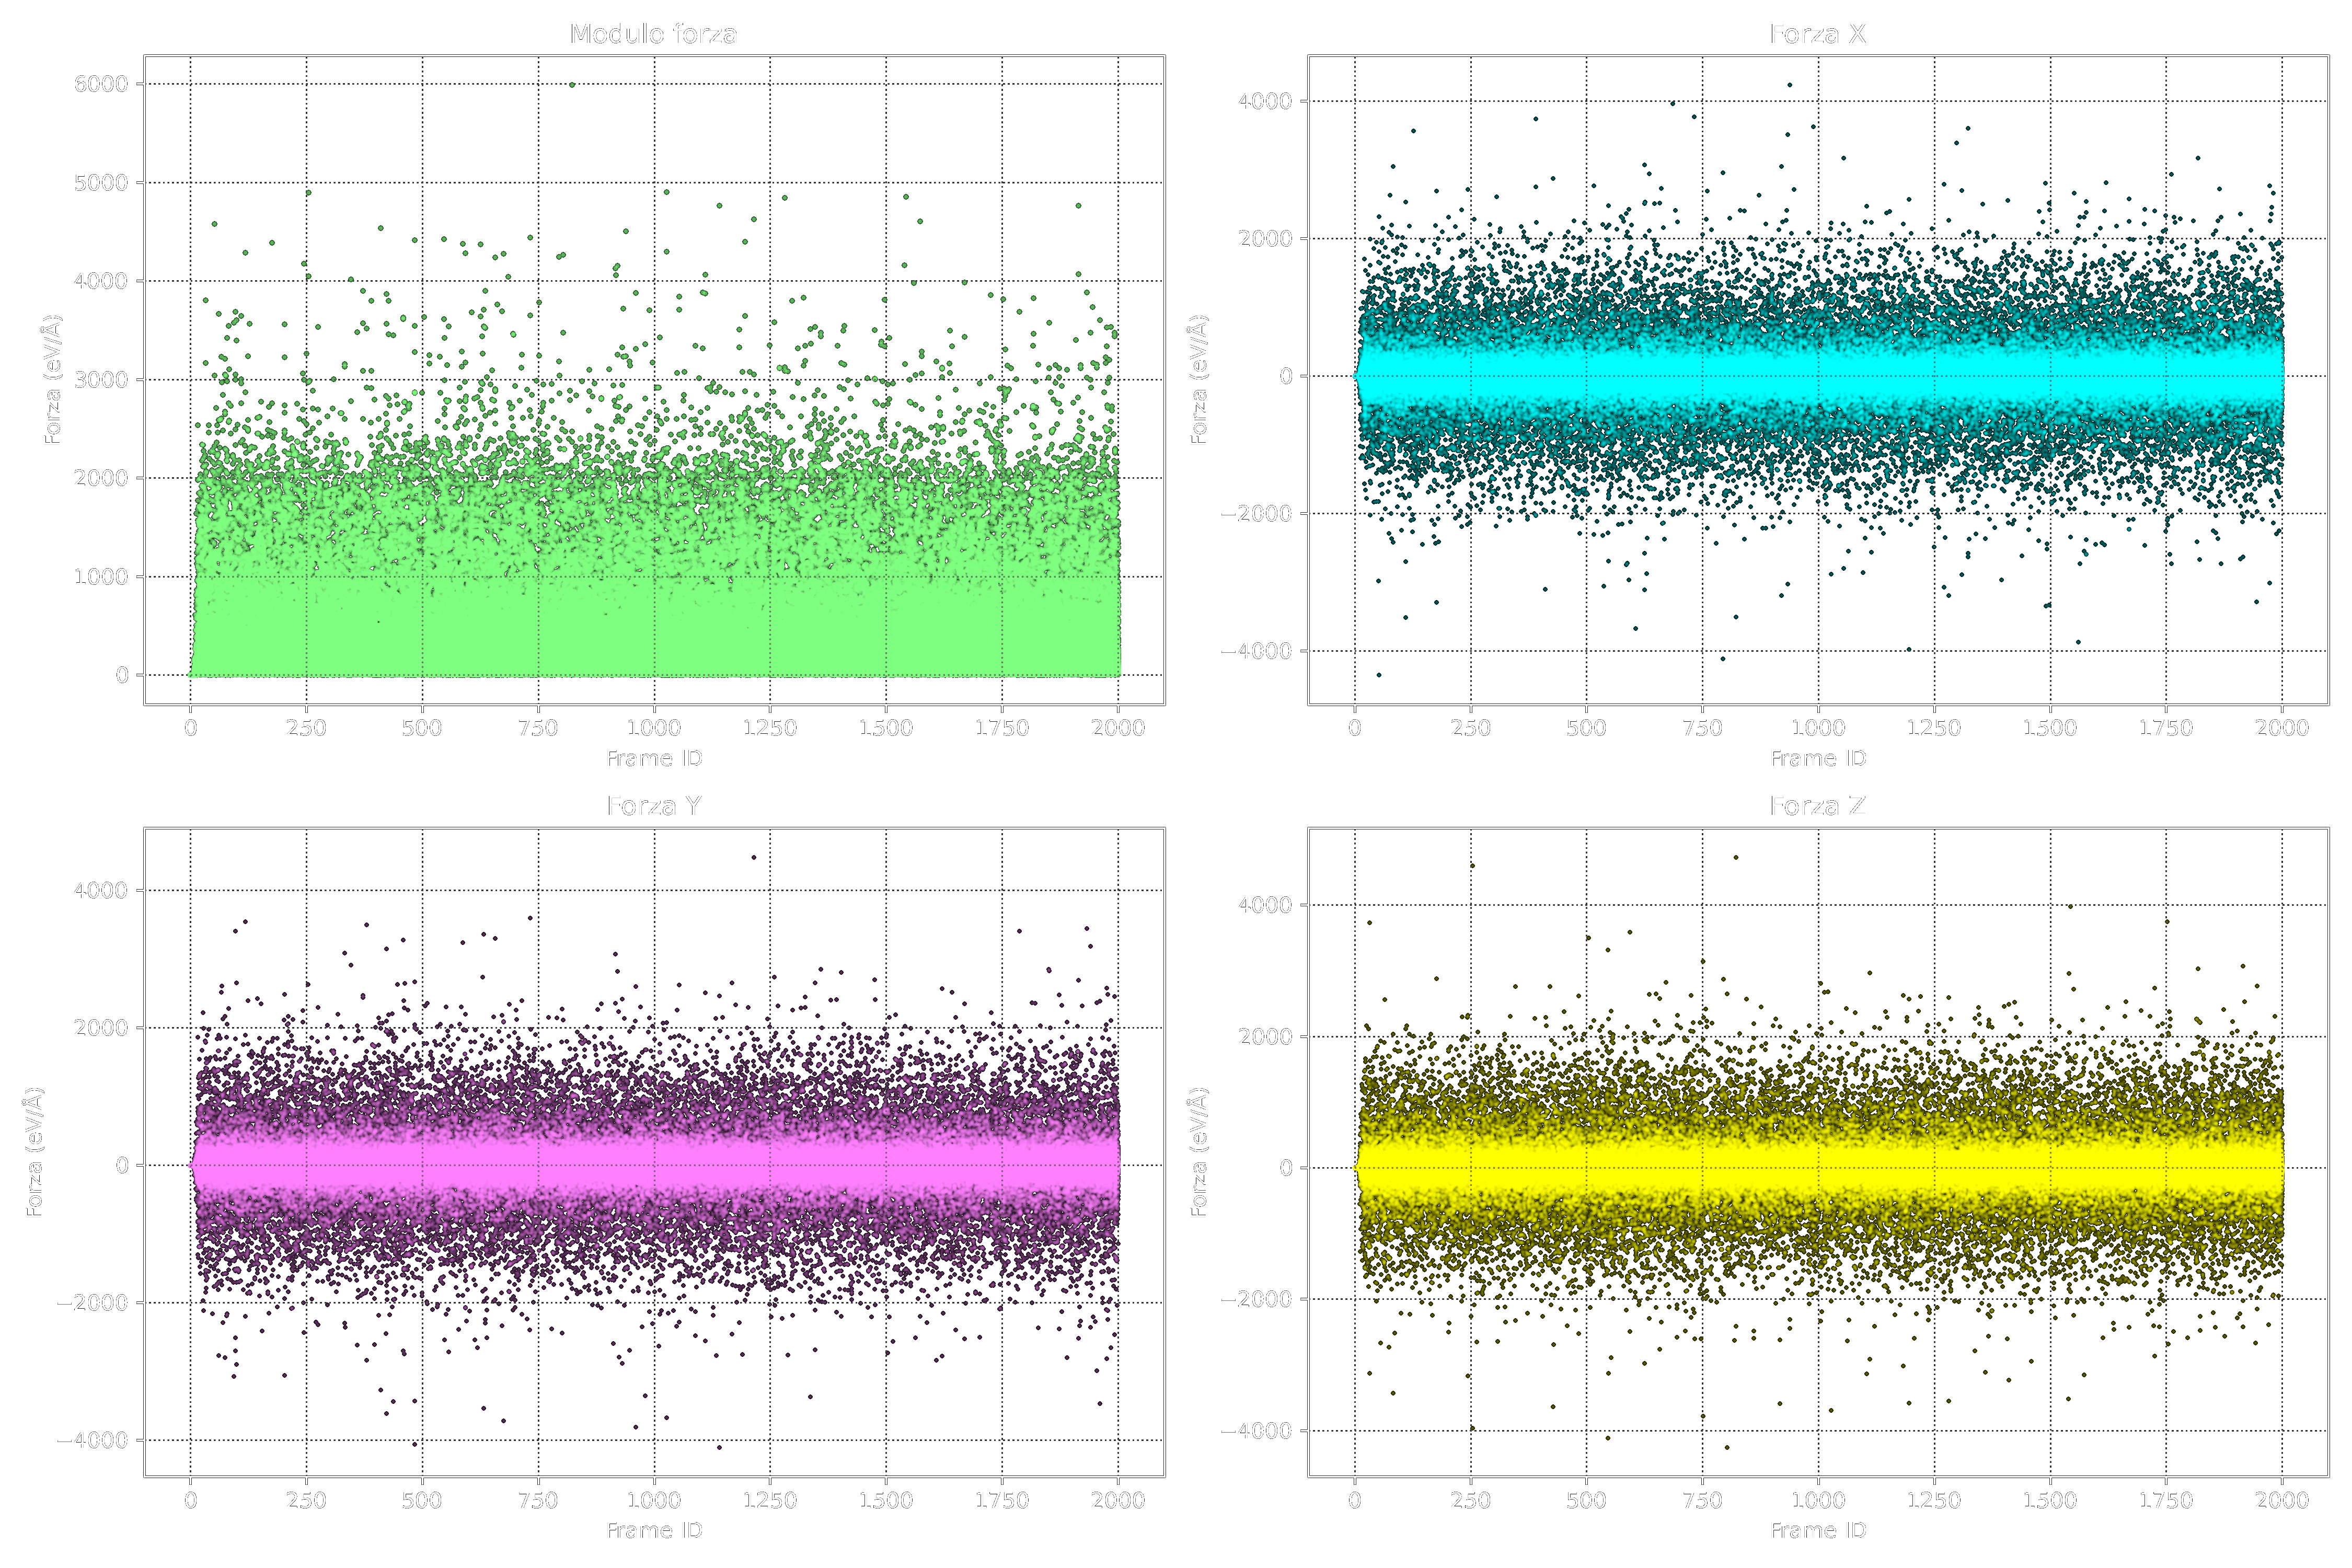
\includegraphics[scale=0.17]{./invnobg/andamento_forze_totali_blocchi_nve_testdata.png}		
		
	\end{column}
\end{columns}
            

\end{frame}



\subsection{NVE: Analisi} %-------------------------------------------------------------------------------------------------------------------
\begin{frame}{Simulazione NVE: analisi}

\begin{columns}[c]        
	% Colonna Sinistra: Testo
	\begin{column}{0.48\textwidth}
		
		\centering
		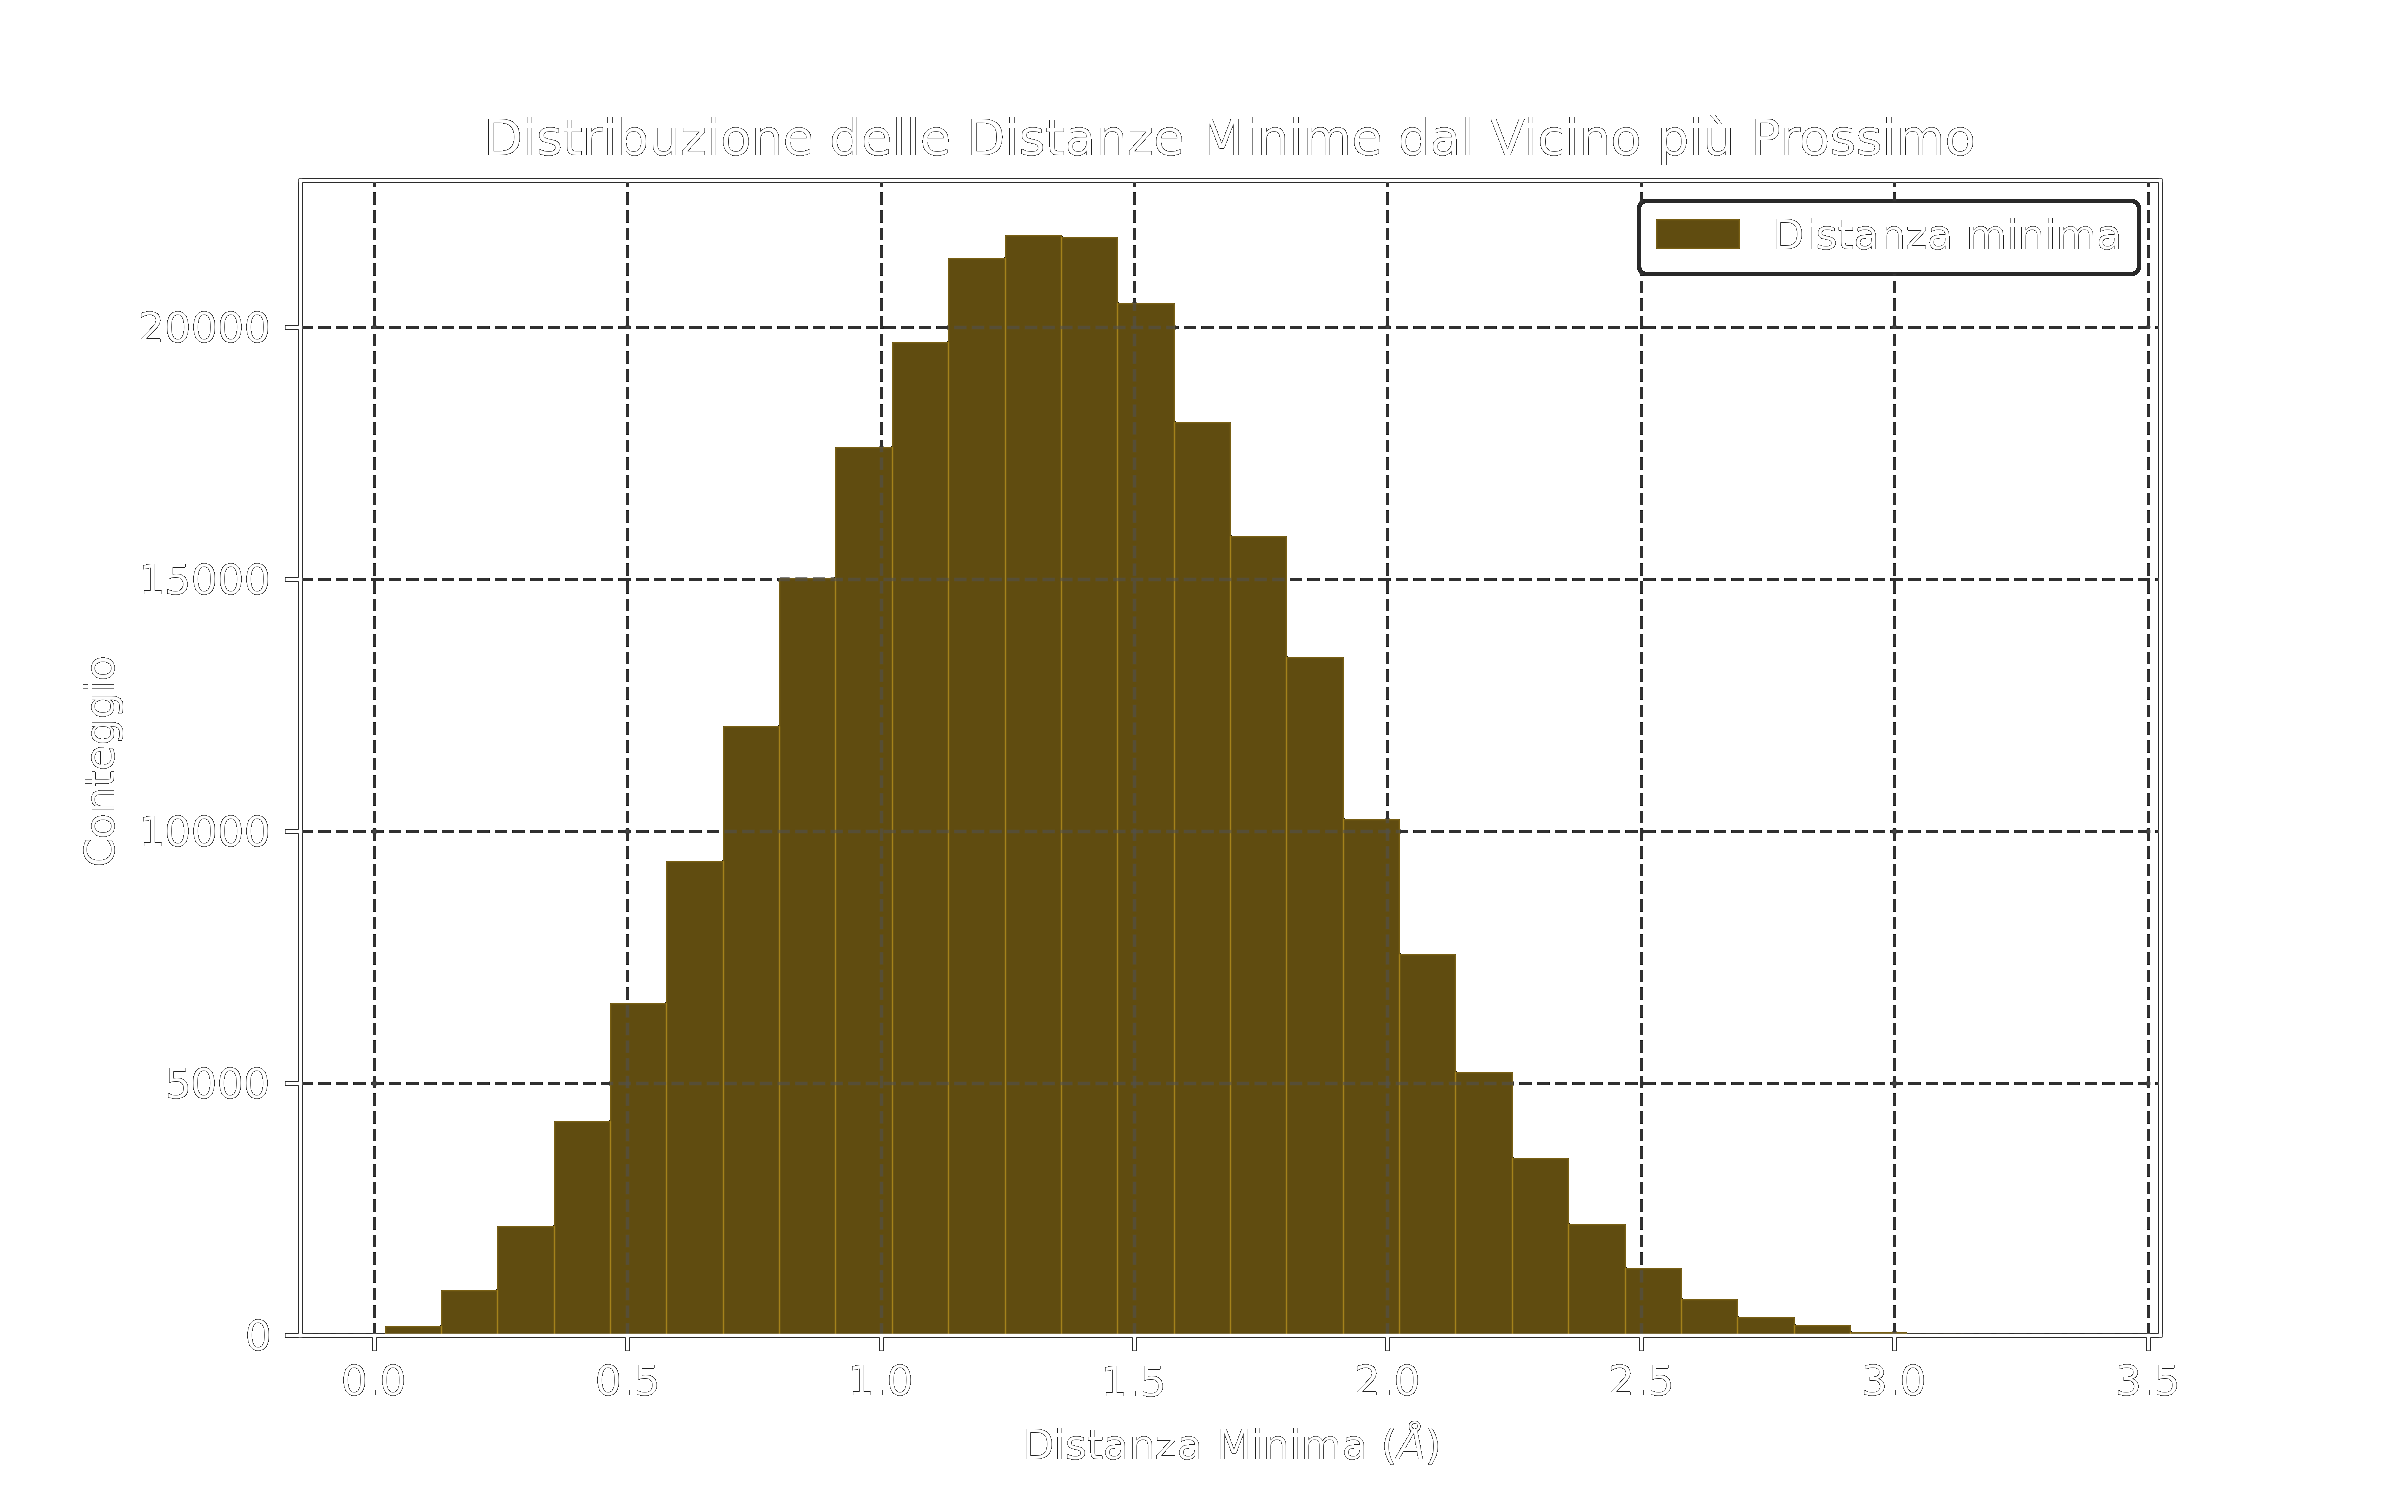
\includegraphics[scale=0.2]{./invnobg/histo_distanze_nve_testdata.png}
		\vspace{0.2em} % Spazio verticale tra le due immagini
		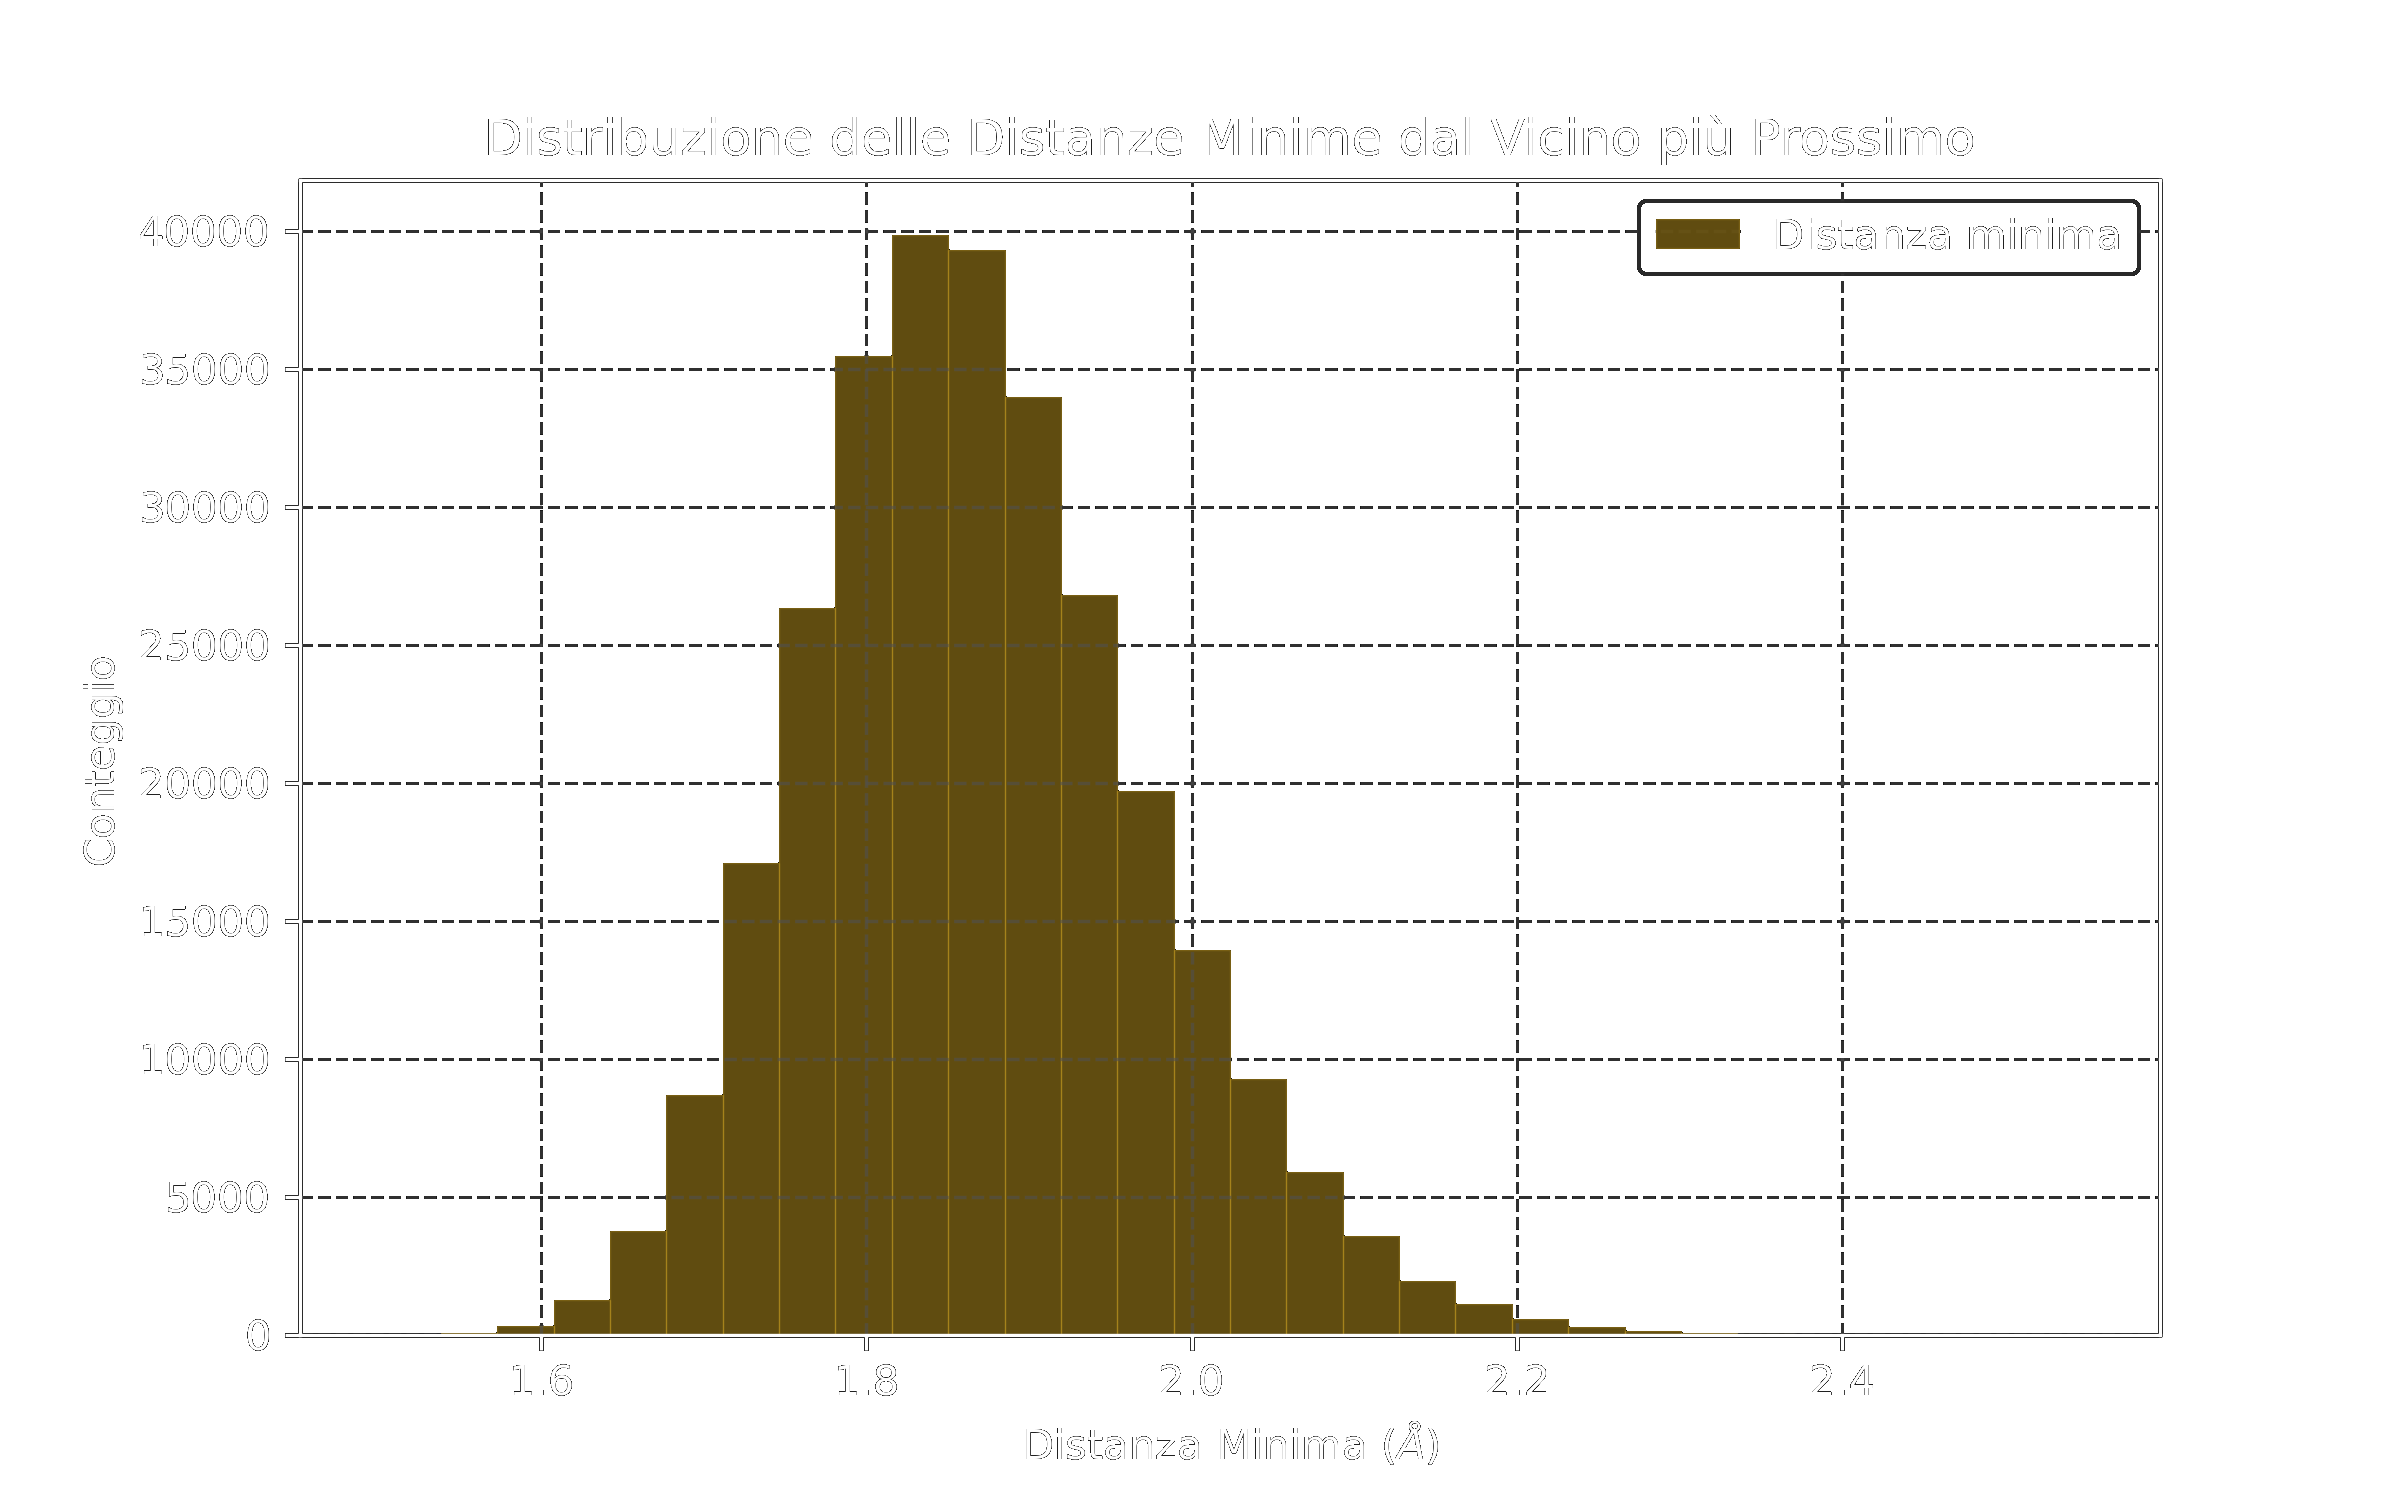
\includegraphics[scale=0.2]{./invnobg/histo_distanze_qe_traindata.png}
		
	\end{column}
	% Colonna Destra: Due immagini incolonnate
	\begin{column}{0.48\textwidth}
		
		\centering
		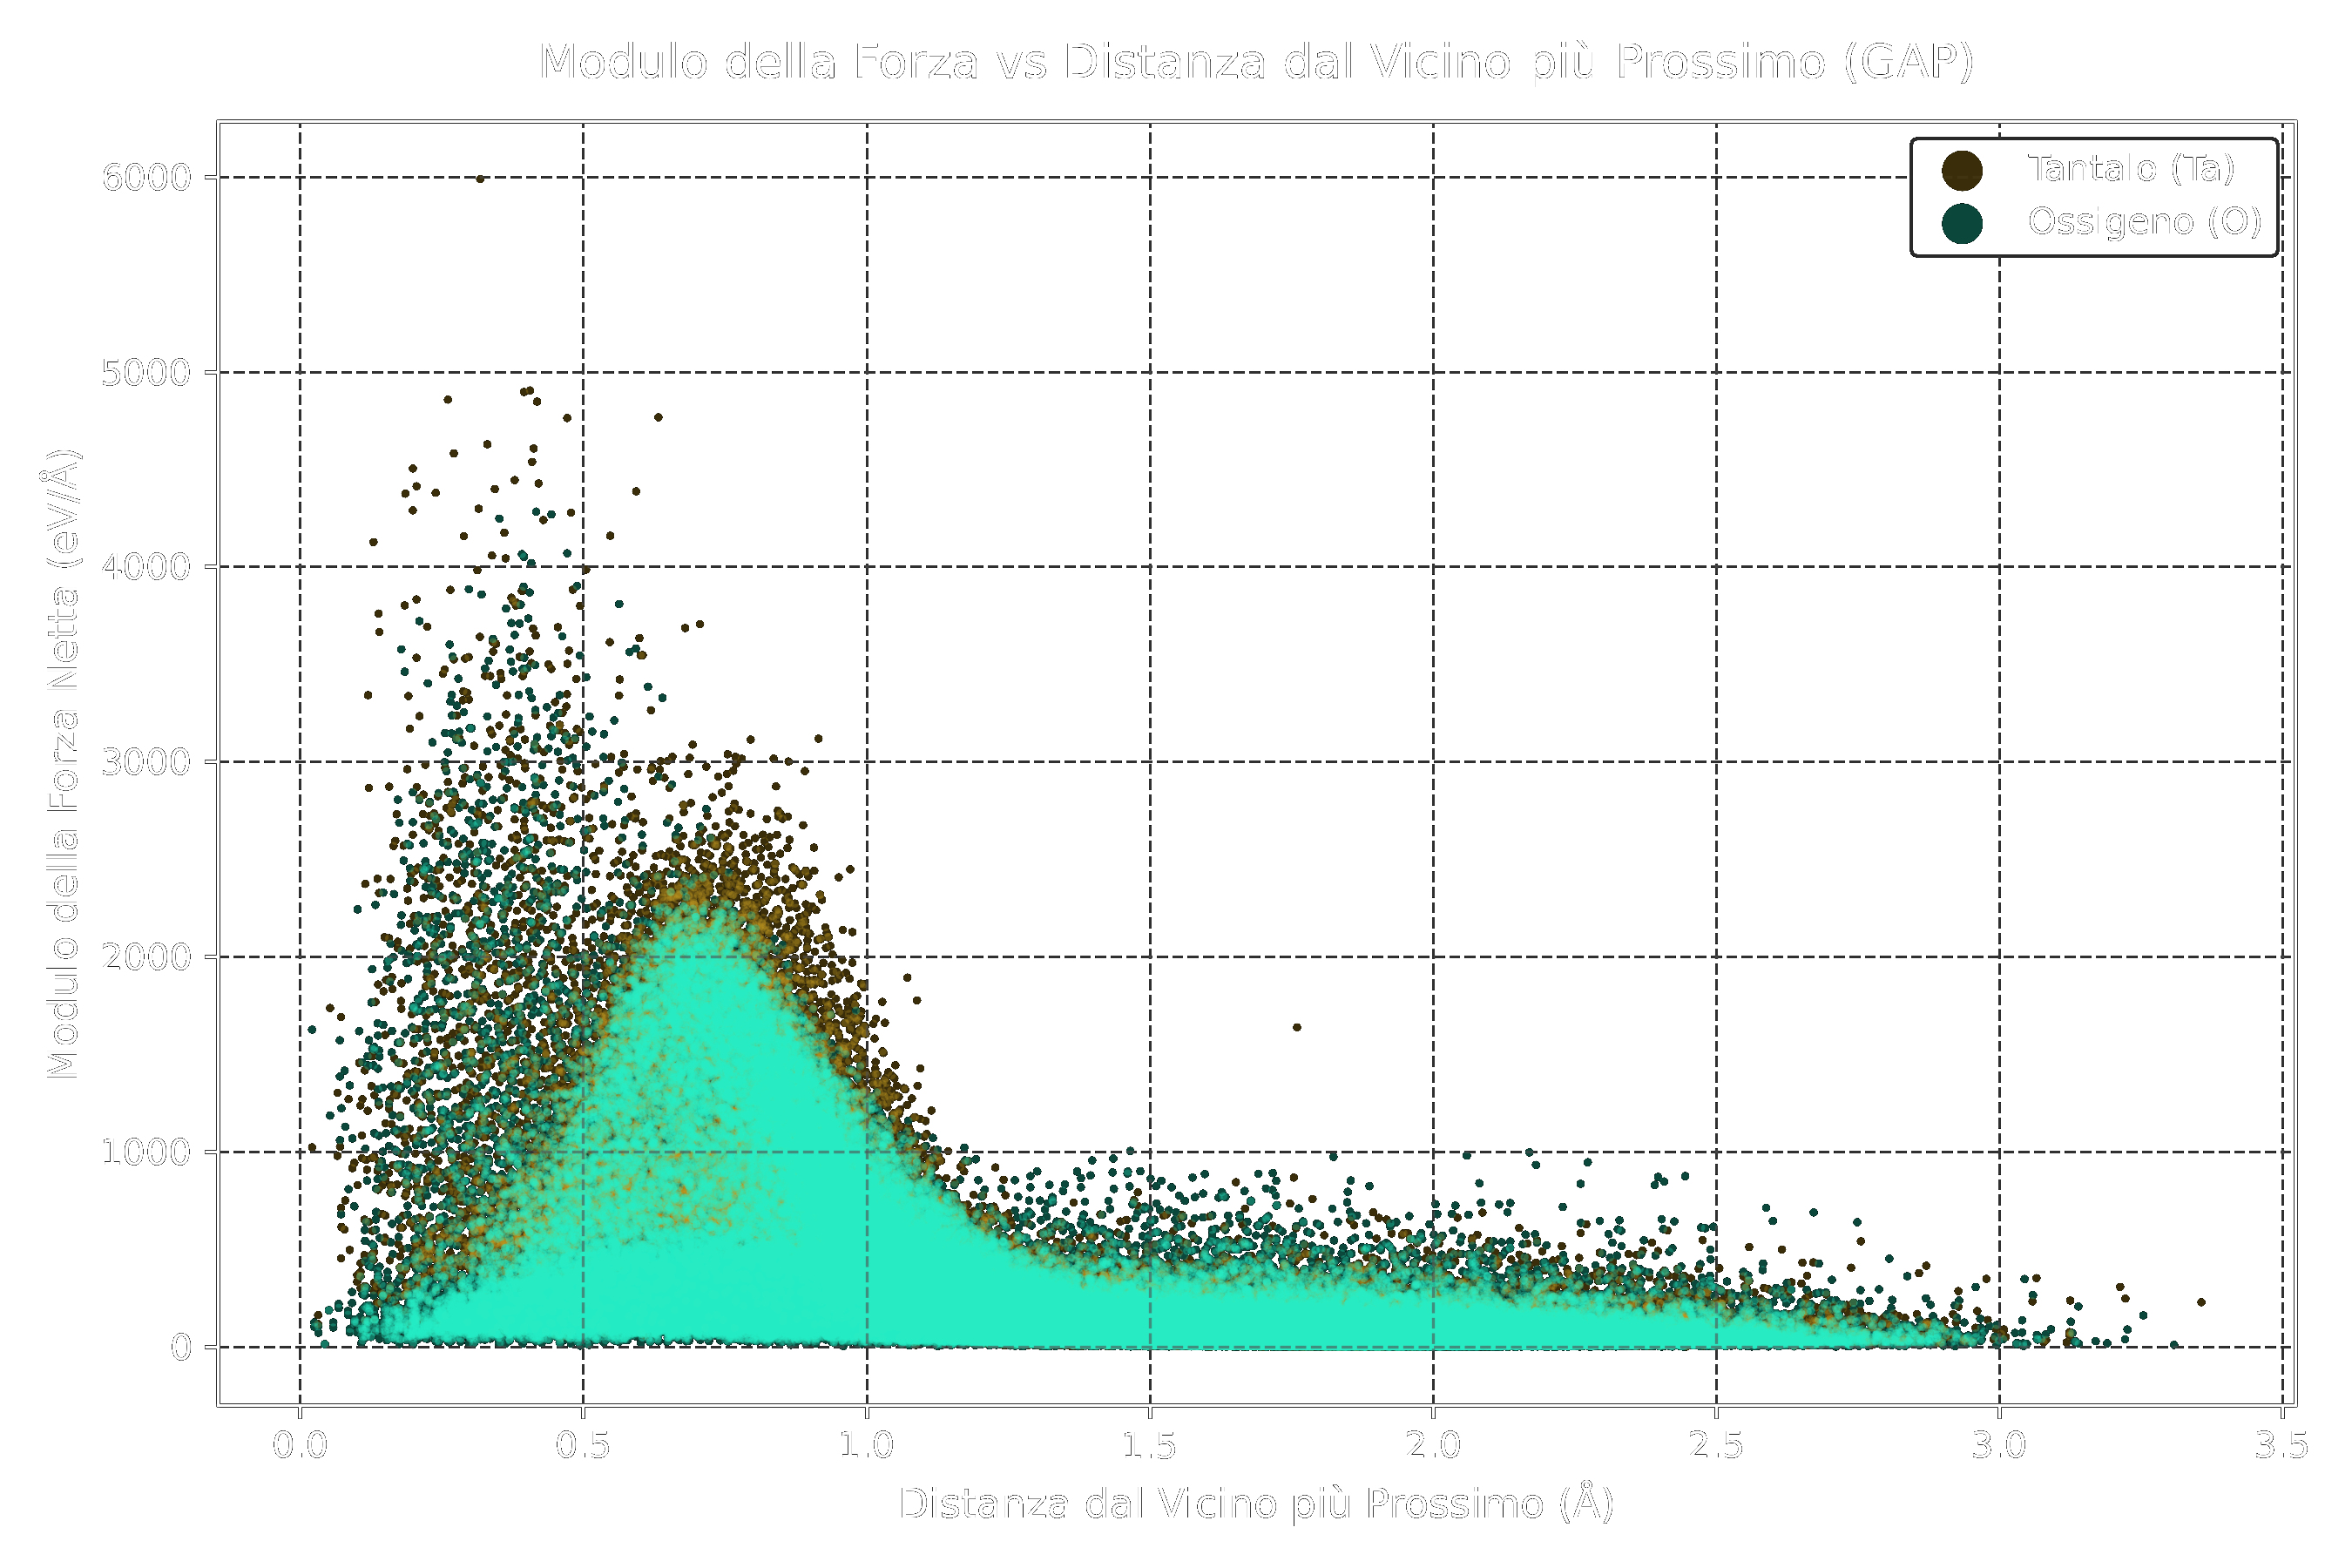
\includegraphics[scale=0.2]{./invnobg/andamento_forze_totali_distanza_nve_testdata.png}		
		\vspace{0.2em} % Spazio verticale tra le due immagini		
		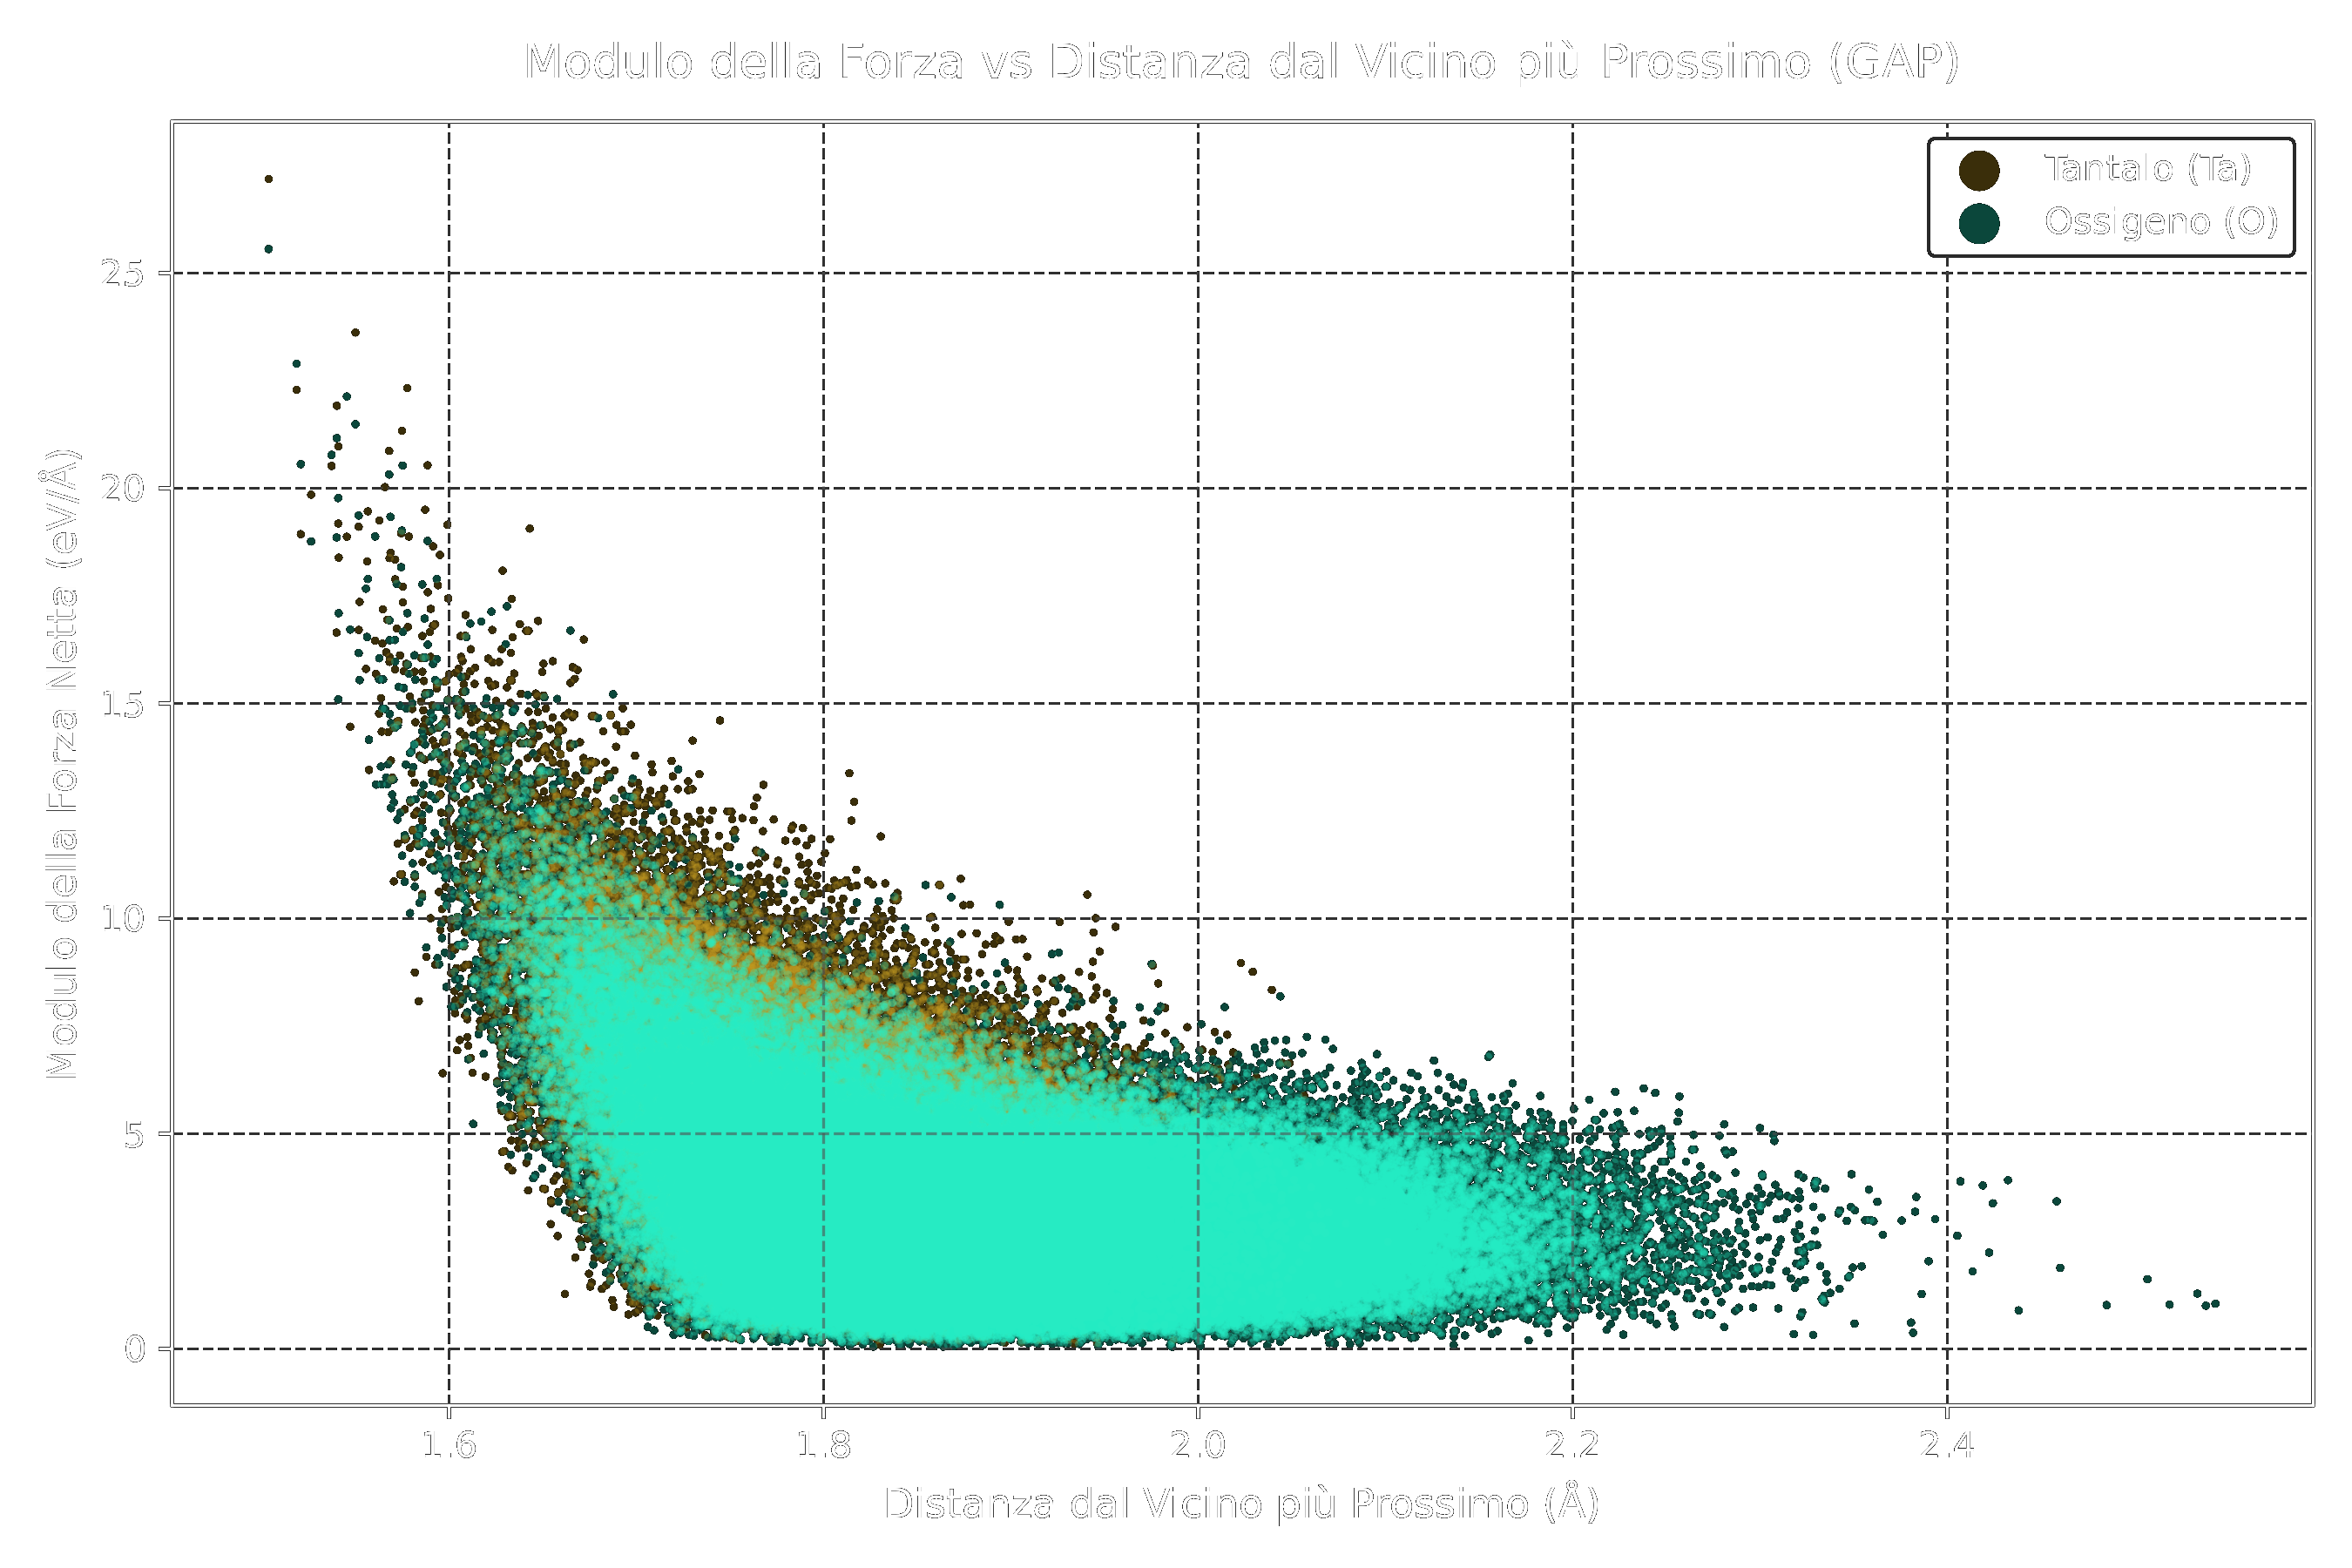
\includegraphics[scale=0.2]{./invnobg/andamento_forze_totali_distanza_qe_traindata.png}
		
	\end{column}
\end{columns}

\end{frame}


\subsection{ZBL} %--------------------------------------------------------------------------------------------------------------------------


\begin{frame}{ZBL: risultati}
    \begin{columns}[c]        
        % Colonna Sinistra: Testo
        \begin{column}{0.48\textwidth}
        
        -----
        
        \end{column}
        % Colonna Destra: Due immagini incolonnate
        \begin{column}{0.48\textwidth}
        
            \centering
            %\includegraphics[height=0.32\paperheight, keepaspectratio]{images/.png}
            
            \vspace{0.4cm} % Spazio verticale tra le due immagini
            
            %\includegraphics[height=0.32\paperheight, keepaspectratio]{images/.png}
            
        \end{column}
    \end{columns}
\end{frame}


\subsection{Algoritmo Metropolis} %----------------------------------------------------------------------------------------------------------


\begin{frame}{Algoritmo di Metropolis: risultati}
	
\begin{columns}[c]        
	% Colonna Sinistra: Testo
	\begin{column}{0.48\textwidth}
		
		\centering
		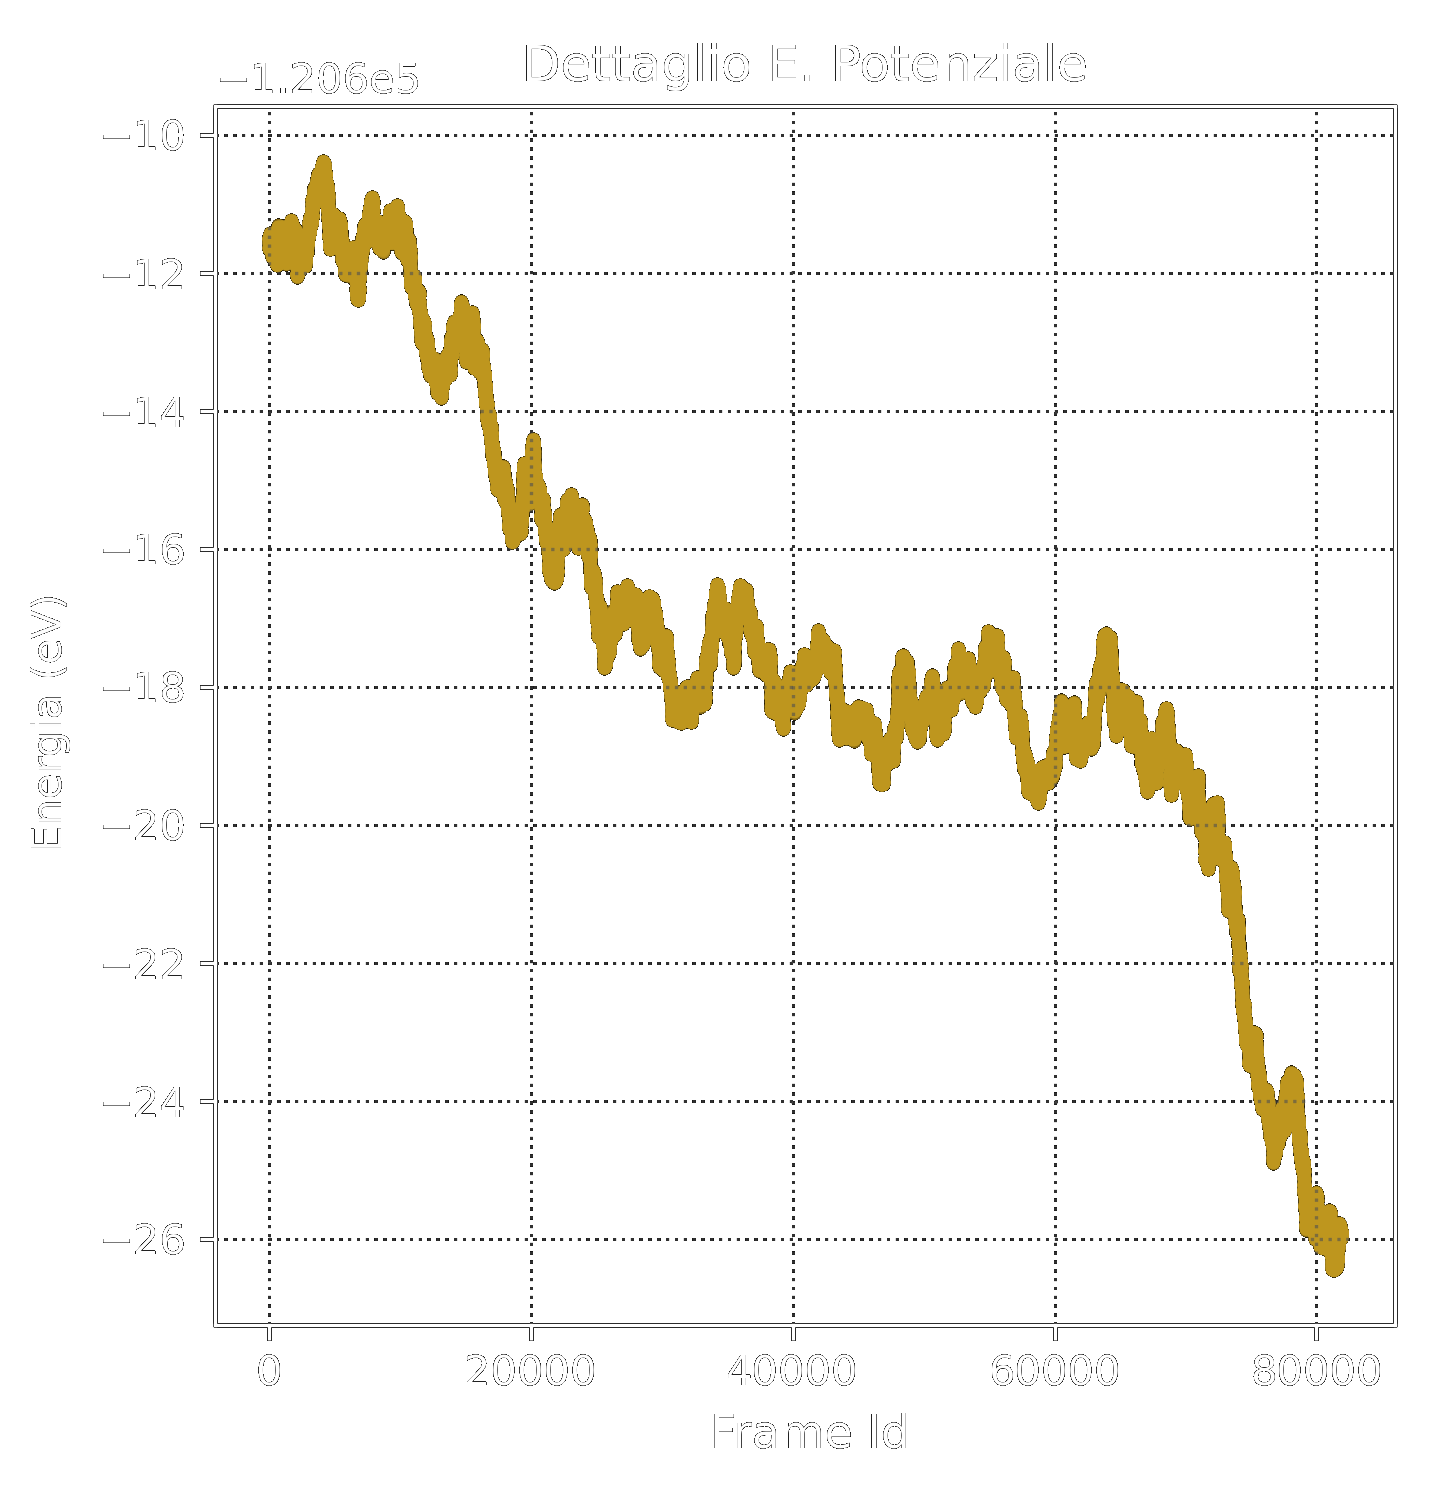
\includegraphics[scale=0.3]{./invnobg/andamento_energia_montecarlo.png}
		
	\end{column}
	% Colonna Destra: Due immagini incolonnate
	\begin{column}{0.48\textwidth}
		
		\centering
		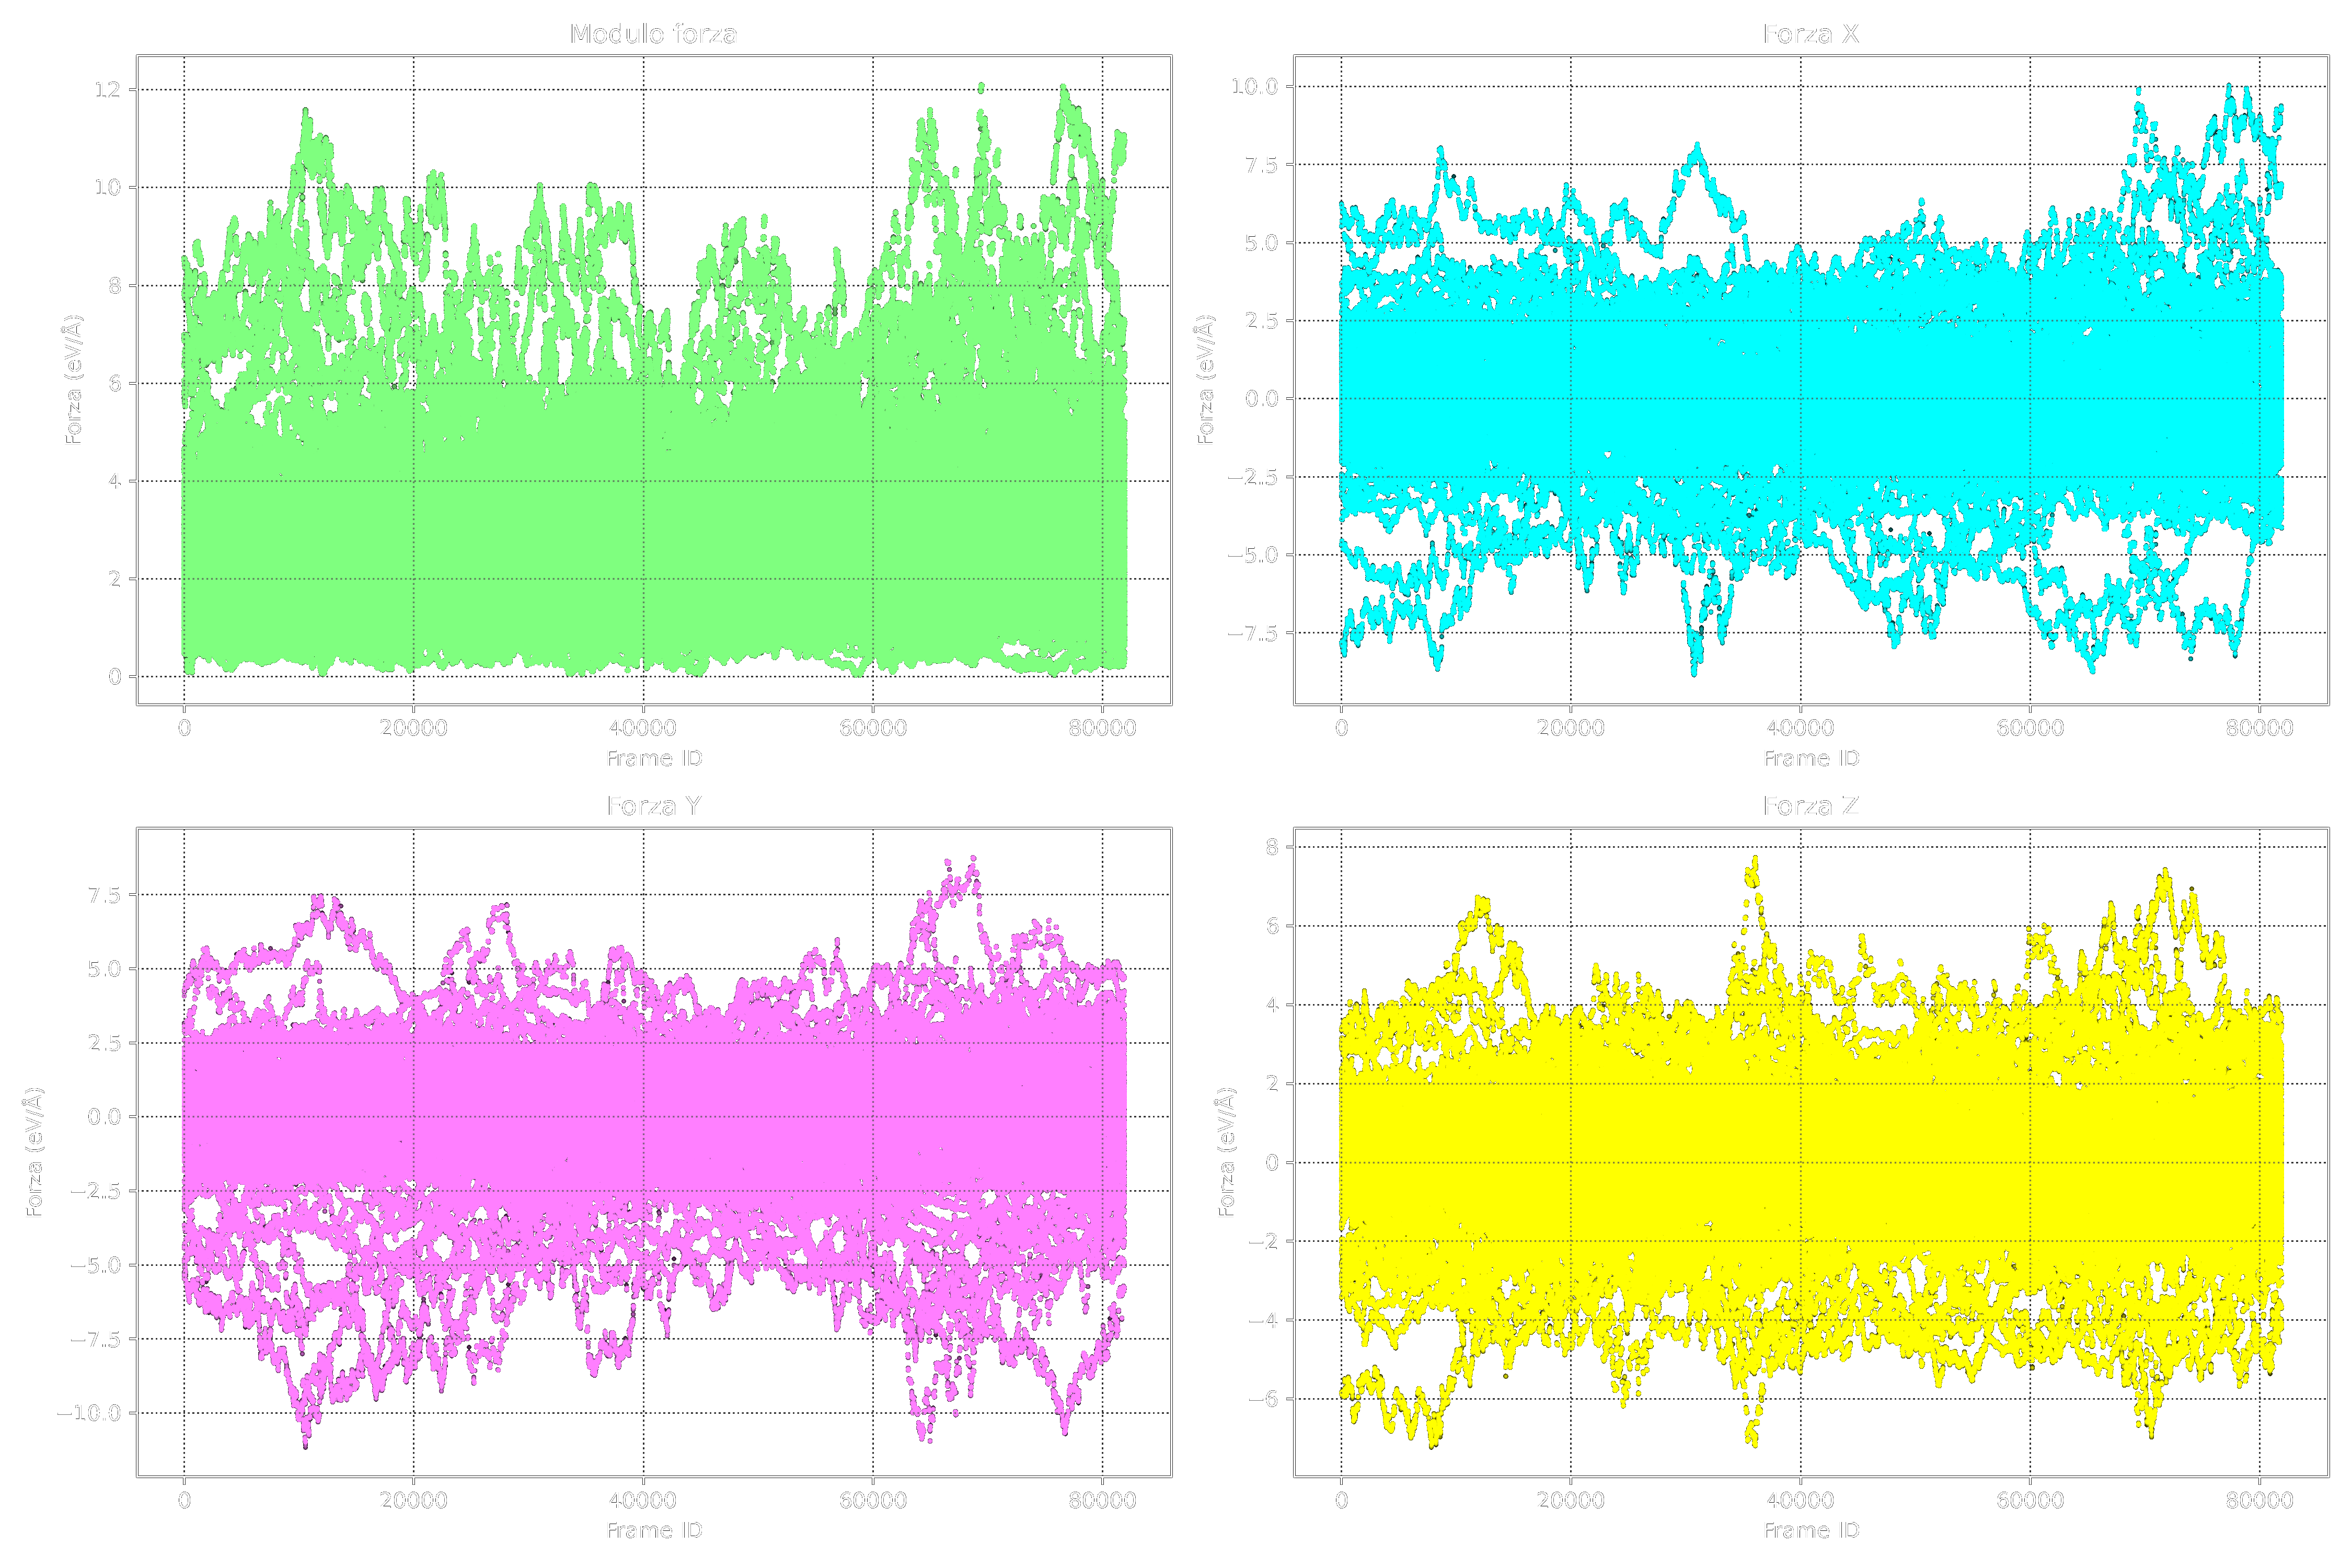
\includegraphics[scale=0.17]{./invnobg/andamento_forze_totali_blocchi_montecarlo.png}
		
	\end{column}
\end{columns}

\end{frame}

\begin{frame}{Algoritmo di Metropolis: risultati}
	
	\begin{columns}[c]        
		% Colonna Sinistra: Testo
		\begin{column}{0.48\textwidth}
			
			\centering
			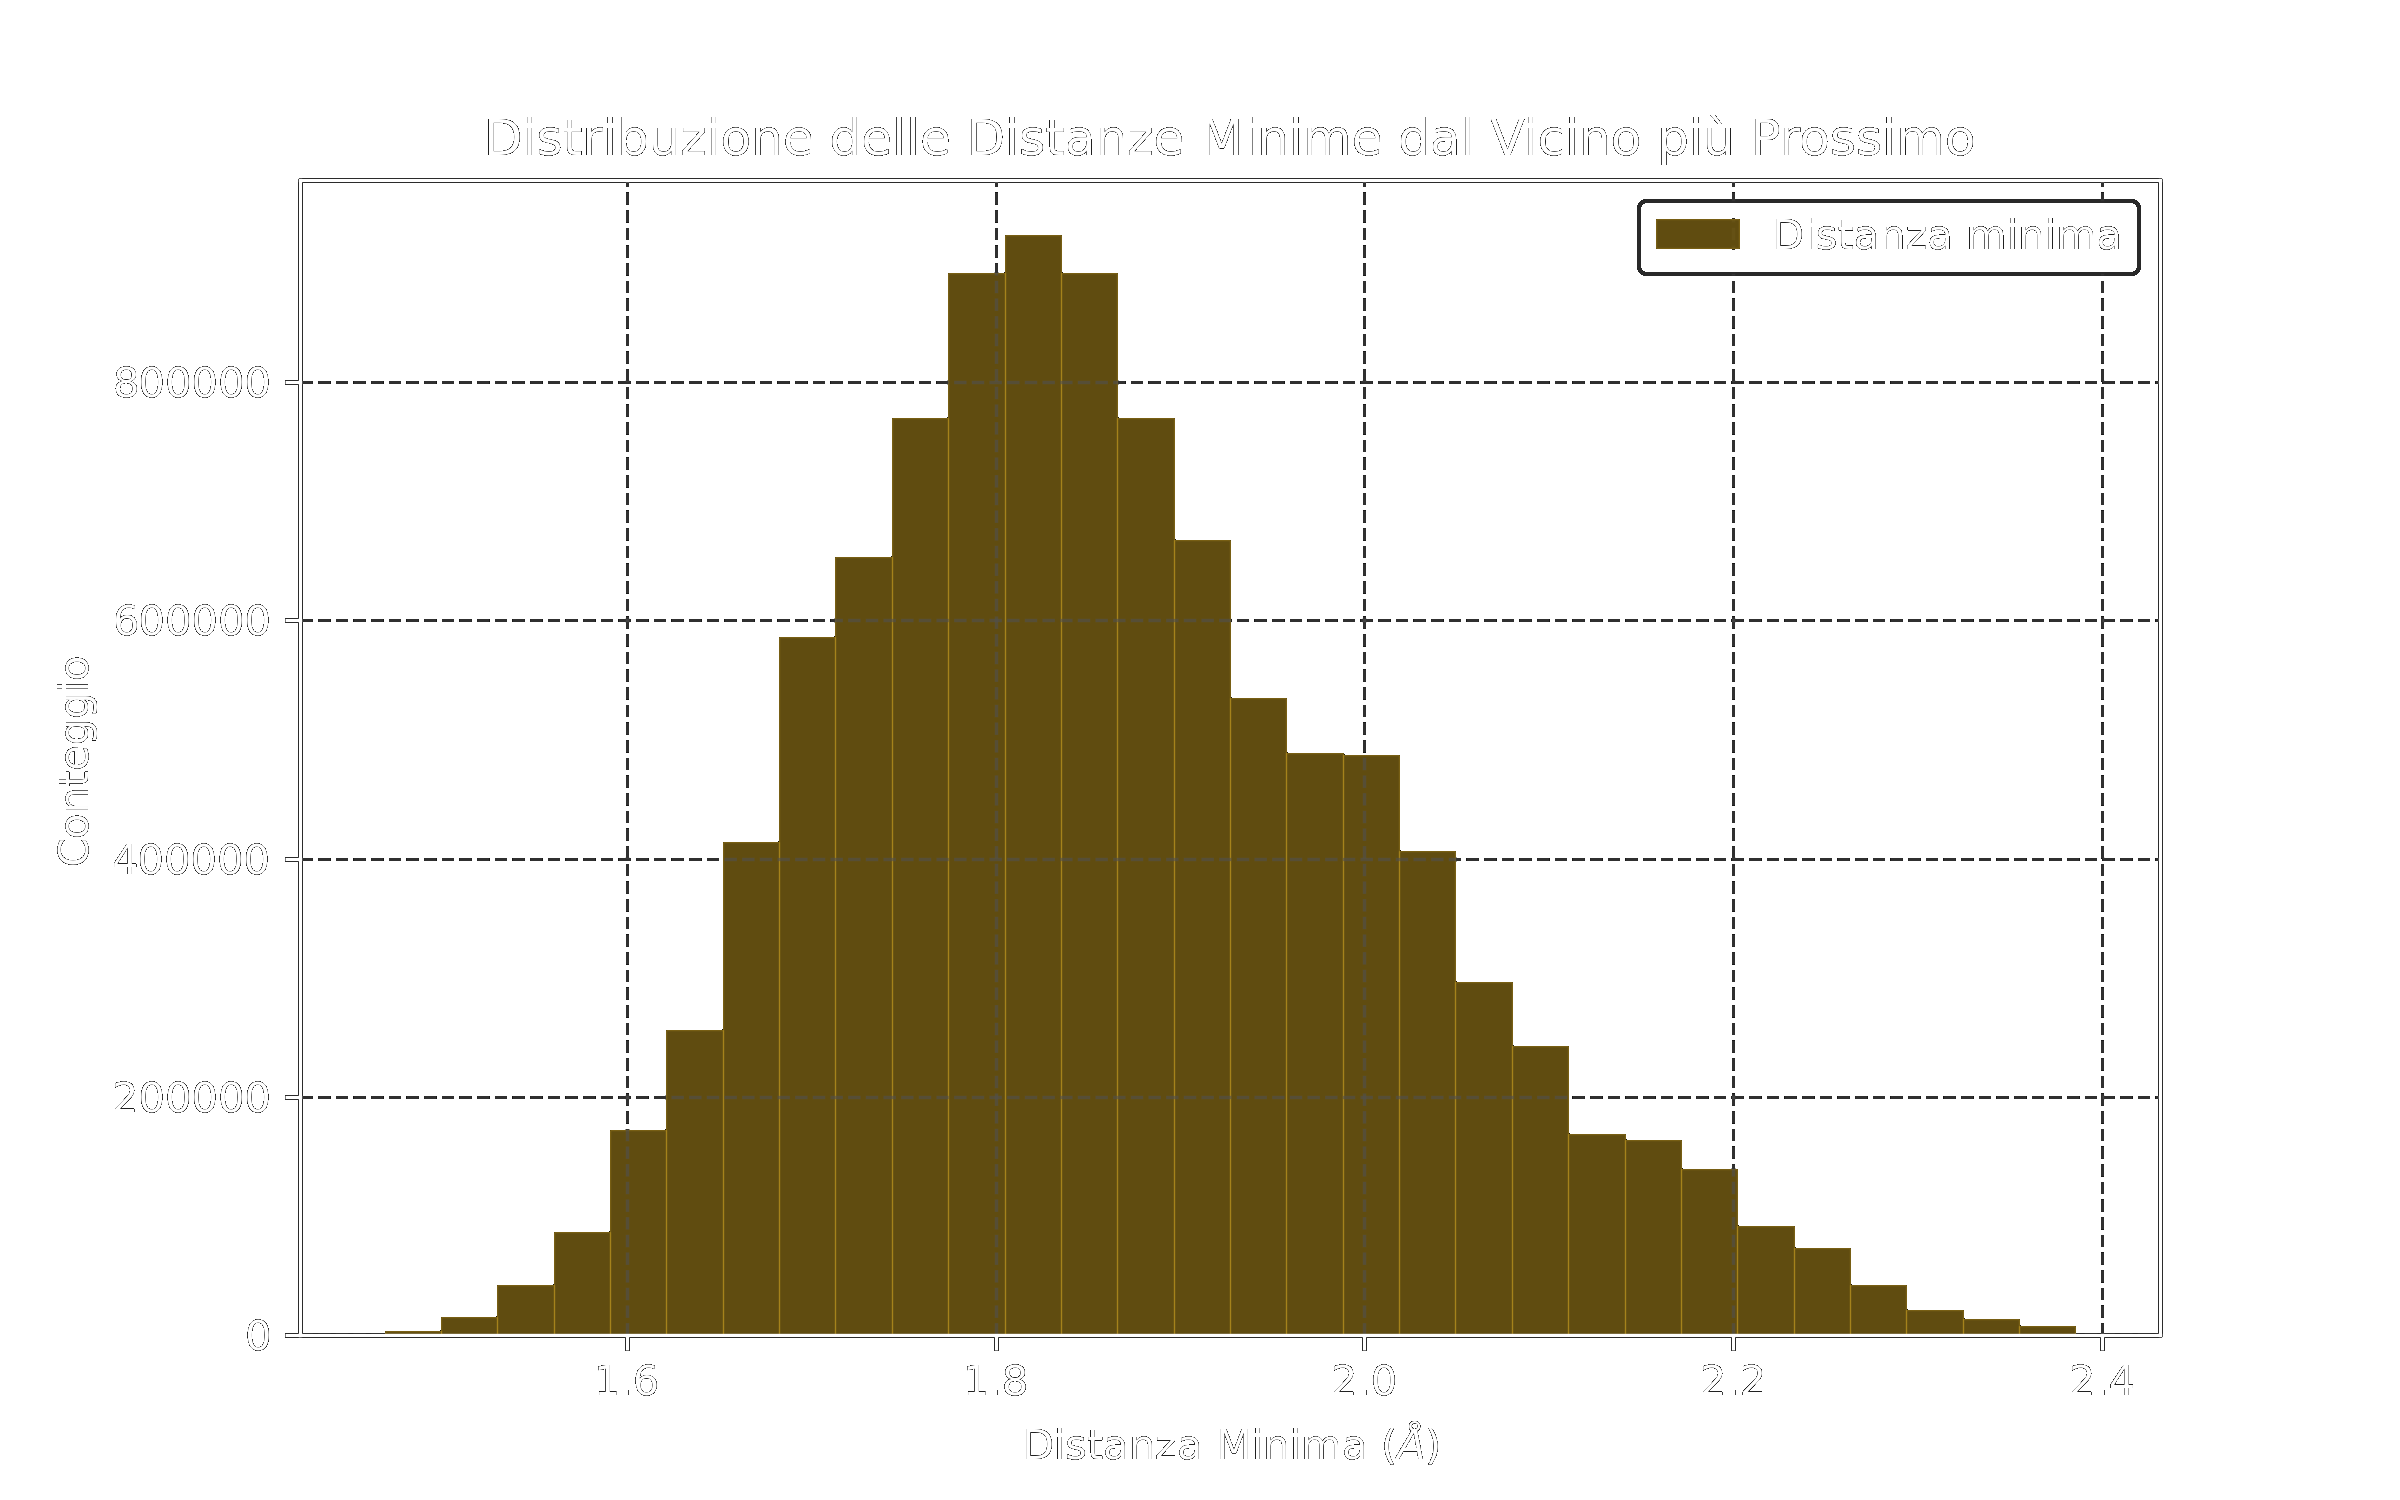
\includegraphics[scale=0.3]{./invnobg/histo_distanze_montecarlo.png}
			
		\end{column}
		% Colonna Destra: Due immagini incolonnate
		\begin{column}{0.48\textwidth}
			
			\centering
			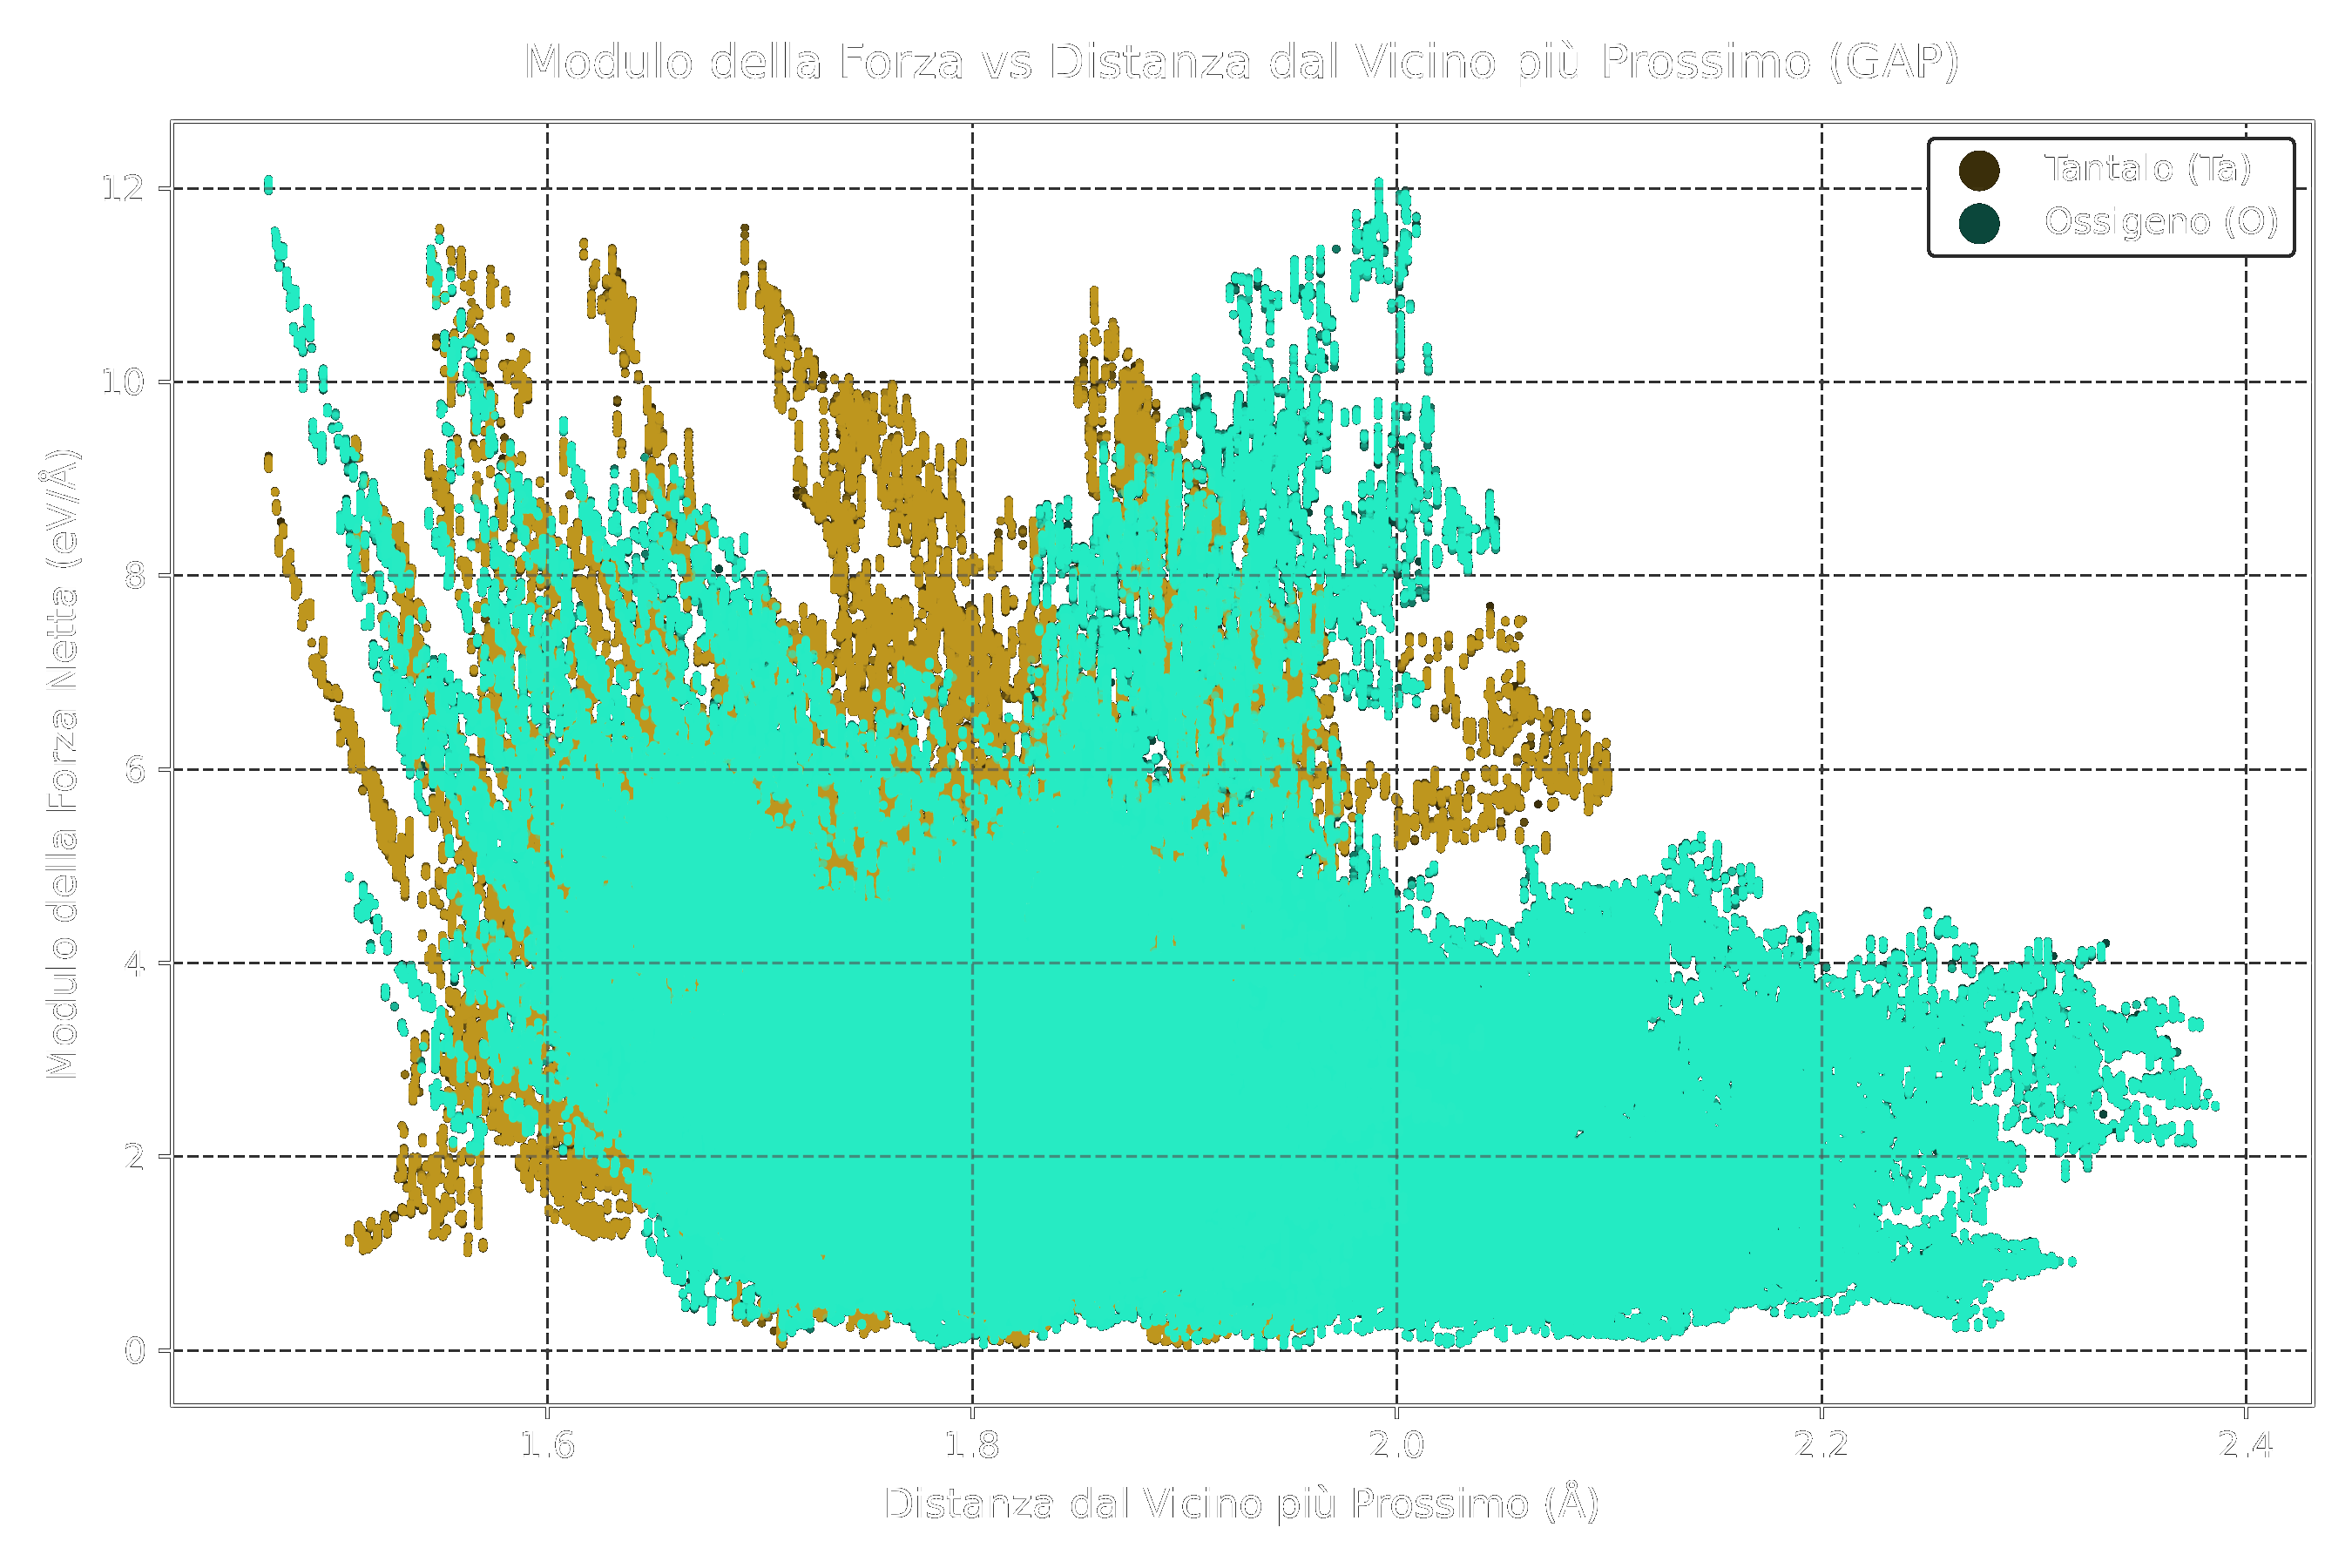
\includegraphics[scale=0.3]{./invnobg/andamento_forze_totali_distanza_montecarlo.png}		
			
		\end{column}
	\end{columns}
	
\end{frame}







